\section{Der Intel 4004}

\begin{frame}
	\frametitle{Der Intel 4004}
	\framesubtitle{Agenda}
	\begin{enumerate}
		\item Der Intel 4004
		\begin{itemize}
			\item Geschichte des MCS-4
			\item MCS-4
			\begin{itemize}
				\item Der 4001
				\item Der 4002
				\item Der 4003
				\item Der 4004
			\end{itemize}
			\item Funktionsweise des 4004
			\item Auswirkungen auf die Prozessorentwicklung
		\end{itemize}
	\end{enumerate}
\end{frame}

\subsection{Geschichte des MCS-4}

\begin{frame}
	\frametitle{Geschichte des MCS-4}
	\framesubtitle{1968 - Gründung von Intel}
	\begin{columns}[c]
		    \begin{column}{.5\textwidth}
		    	\begin{itemize}
		    		\item Gegründet von Gordon E. Moore und Robert Noyce
		    		\item Hersteller von Speicherchips auf Halbleiterbasis
		    		\item Problem: Kunden zögerten von magnetischen Speichern zu wechseln
		    	\end{itemize}
		    \end{column}
		    \begin{column}{.5\textwidth}
		    	\begin{figure}
		    	    \includegraphics[width=0.7\linewidth]{images/old_intel_logo.png}
		    	\end{figure}
		    \end{column}
	\end{columns}
\end{frame}

\begin{frame}
	\frametitle{Geschichte des MCS-4}
	\framesubtitle{1969 - Auftrag von Busicom}
	\begin{columns}[c]
		\begin{column}{.5\textwidth}
			\begin{itemize}
				\item Spezialauftrag für Busicoms Rechenmaschine
				\item Erstes Design:
				\begin{itemize}
					\item 7 - 12 Chips mit geschätzt 3000 - 5000 Transistoren und 40 Pins
					\item Schieberegister Speicher
					\item komplexes Makroinstruktionsset
				\end{itemize}
				\item Intel hatte keine Erfahrung mit Design von Logikchips
			\end{itemize}
		\end{column}
		\begin{column}{.5\textwidth}
			\begin{figure}[ht]
				 \includegraphics[width=0.8\linewidth]{images/unicom_141P.jpg}
				\caption{Busicom Unicom 141P }
			\end{figure}
		\end{column}
	\end{columns}
\end{frame}

\begin{frame}
	\frametitle{Geschichte des MCS-4}
	\framesubtitle{Neues Design von Intel}
	\begin{columns}[c]
		\begin{column}{.5\textwidth}
			\begin{itemize}
				\item Reduzierung der Komplexität mit Hilfe von größerem Speicher
				\item Mikroinstruktionen
				\item 4-bit Binary Coded Decimal Arithmetik
				\item 3 Chip Design bestehend aus CPU, RAM und ROM
				\item 1900 Transistoren pro Chip
				\item Vergleich zweites Busicom Design: 12 Chips mit 2000 Transistoren und 40 Pins
			\end{itemize}
		\end{column}
		\begin{column}{.5\textwidth}
			\begin{table}[h]
				\begin{tabular}{cc}
					\includegraphics[width=0.35\linewidth]{images/hoff.jpeg}
					%Marcian Edward "Ted" Hoff, Jr.
					& 	
					\includegraphics[width=0.35\linewidth]{images/mazor.jpg}
					%Stanley "Stan" Mazor
					\\
					\includegraphics[width=0.4\linewidth]{images/shima.jpeg}
					% Masatoshi Shima
					& 		\includegraphics[width=0.35\linewidth]{images/faggin.jpg}
					% Federico Faggin
				\end{tabular}
			\end{table}
		\end{column}
	\end{columns}
\end{frame}

\begin{frame}
	\frametitle{Geschichte des MCS-4}
	\framesubtitle{1970 - Entscheidung und Produktion}
	\begin{columns}
		\begin{column}{.5\textwidth}	
				\begin{itemize}
					\item Busicom entscheidet sich Intels Designvorschlag anzunehmen
					\item Intel stellt Federico Faggin als Logik- und Chipdesigner ein
					\item Masatoshi Shima arbeitet an den ersten Programmen für den neuen Prozessor
					\item erster Prototyp nach 9 Monaten fertig
				\end{itemize}
		\end{column}
		\begin{column}{.5\textwidth}
			\begin{figure}[ht]
				\includegraphics[width=1\linewidth]{images/intel_chips.jpg}
				\caption{Intel MCS-4}
			\end{figure}
		\end{column}
	\end{columns}
\end{frame}

\subsection{MCS-4}

\subsubsection{Der 4001}
\begin{frame}
	\frametitle{Der 4001}
	\framesubtitle{Programmierbarer ROM}
	\begin{columns}
		\begin{column}{.5\textwidth}	
			\begin{itemize}
				\item Programmspeicher
				\item 2048 bits als 256 8-bit Wörter
				\item maximal 16 ROMs hintereinander schaltbar
				\item 2. Operationsmodus: I/O Befehle
			\end{itemize}
		\end{column}
		\begin{column}{.6\textwidth}
			\begin{figure}[ht]
				\includegraphics[width=1\linewidth]{images/layout_4001.png}
			\end{figure}
		\end{column}
	\end{columns}
\end{frame}

\subsubsection{Der 4002}
\begin{frame}
	\frametitle{Der 4002}
	\framesubtitle{Random-Access Memory}
	\begin{columns}
		\begin{column}{.5\textwidth}	
			\begin{itemize}
				\item 2 Versionen: 4002-1 und 4002-2
				\item Datenspeicher für Berechnungen
				\item 320 bits als 4 Register von 20 4-bit character
				\begin{itemize}
					\item 16 Daten character
					\item 4 Status character
				\end{itemize}
			\end{itemize}
		\end{column}
		\begin{column}{.6\textwidth}
			\begin{figure}[ht]
				\includegraphics[width=1.1\linewidth]{images/layout_4002.png}
			\end{figure}
		\end{column}
	\end{columns}
\end{frame}

\subsubsection{Der 4003}
\begin{frame}
	\frametitle{Der 4003}
	\framesubtitle{I/O Schieberegister}
	\begin{columns}
		\begin{column}{.5\textwidth}	
			\begin{itemize}
				\item 10-bit statisches Schieberegister
				\item Eingabe: seriell
				\item Ausgabe: seriell, parallel
				\item Erweitert ROM und RAM I/O Ports
				\item Können hintereinander geschaltet werden
				\item Ermöglicht das Anschließen von Tastaturen, Displays, Druckern, etc
			\end{itemize}
		\end{column}
		\begin{column}{.6\textwidth}
			\begin{figure}[ht]
				\includegraphics[width=1.1\linewidth]{images/layout_4003.png}
			\end{figure}
		\end{column}
	\end{columns}
\end{frame}

\subsubsection{Der 4004}

\begin{frame}
	\frametitle{Der 4004}
	\framesubtitle{Die CPU}
	\begin{columns}
		\begin{column}{.5\textwidth}	
			\begin{itemize}
				\item 4 funktionale Blöcke
				\begin{itemize}
					\item Adressregister
					\item Indexregister
					\item 4-bit Addierer
					\item Instruktionsregister
				\end{itemize}
			\end{itemize}
		\end{column}
		\begin{column}{.5\textwidth}
			\begin{figure}[ht]
				\includegraphics[width=1\linewidth]{images/pins_4004.png}
			\end{figure}
		\end{column}
	\end{columns}
\end{frame}

\begin{frame}
	\frametitle{Der 4004}
	\framesubtitle{Detailansicht des 4004}
			\begin{figure}[ht]
				\includegraphics[width=0.7\linewidth]{images/layout_4004.png}
			\end{figure}
\end{frame}

\begin{frame}
	\frametitle{Der 4004}
	\framesubtitle{Detailansicht des 4004}
	\begin{figure}[ht]
		\includegraphics[width=0.7\linewidth]{images/layout_4004_1.png}
	\end{figure}
\end{frame}

\begin{frame}
	\frametitle{Der 4004}
	\framesubtitle{Adressregister}
	\begin{columns}
		\begin{column}{.5\textwidth}
			\begin{itemize}
				\item 4 12bit Register
				\item Organisiert als Stack
				\item Speichert die aktuelle Programmadresse
				\item Zusätzliche 3 Level für Subroutinen
			\end{itemize}
		\end{column}
		\begin{column}{.5\textwidth}
			\begin{figure}[ht]
				\includegraphics[width=0.5\linewidth]{images/addr_register.png}
			\end{figure}
		\end{column}
	\end{columns}
\end{frame}

\begin{frame}
	\frametitle{Der 4004}
	\framesubtitle{Detailansicht des 4004}
	\begin{figure}[ht]
		\includegraphics[width=0.7\linewidth]{images/layout_4004_2.png}
	\end{figure}
\end{frame}

\begin{frame}
	\frametitle{Der 4004}
	\framesubtitle{Indexregister}
	\begin{columns}
		\begin{column}{.5\textwidth}
			\begin{itemize}
				\item Organisiert in 8 Reihen mit jeweils 8 bit
				\item Möglichkeit eine Reihe von 8bit oder jedes Wort einzeln auszulesen
				\item Cache für Zwischenergebnisse oder Instruktionen
			\end{itemize}
		\end{column}
		\begin{column}{.5\textwidth}
			\begin{figure}[ht]
				\includegraphics[width=0.6\linewidth]{images/index_register.png}
			\end{figure}
		\end{column}
	\end{columns}
\end{frame}

\begin{frame}
	\frametitle{Der 4004}
	\framesubtitle{Detailansicht des 4004}
	\begin{figure}[ht]
		\includegraphics[width=0.7\linewidth]{images/layout_4004_3.png}
	\end{figure}
\end{frame}

\begin{frame}
	\frametitle{Der 4004}
	\framesubtitle{4-bit Addierer}
	\begin{columns}
		\begin{column}{.5\textwidth}
			\begin{itemize}
				\item Kann sowohl in binär als auch in BCD Arithmetik rechnen
				\item Erster Term aus einem internen Bufferregister
				\item Carry und 2. Term aus dem Akkumulator
				\item Ergebnis wird im Akkumulator gespeichert
			\end{itemize}
		\end{column}
		\begin{column}{.5\textwidth}
			\begin{figure}
				\begin{figure}[ht]
					\includegraphics[width=0.6\linewidth]{images/adder.png}
				\end{figure}
			\end{figure}
		\end{column}
	\end{columns}
\end{frame}

\begin{frame}
	\frametitle{Der 4004}
	\framesubtitle{Detailansicht des 4004}
	\begin{figure}[ht]
		\includegraphics[width=0.7\linewidth]{images/layout_4004_4.png}
	\end{figure}
\end{frame}

\begin{frame}
	\frametitle{Der 4004}
	\framesubtitle{Instruktionsregister}
	\begin{columns}
		\begin{column}{.5\textwidth}
			\begin{itemize}
				\item OPR und OPA
				\item Enthält die aktuelle Instruktion
				\item Enthält zusätzliche Einheit zur Dekodierung von Instruktionen
			\end{itemize}
		\end{column}
		\begin{column}{.5\textwidth}
			\begin{figure}[ht]
				\includegraphics[width=0.3\linewidth]{images/instruction_register.png}
			\end{figure}
		\end{column}
	\end{columns}
\end{frame}

\subsection{Funktionsweise des 4004}

\begin{frame}
	\frametitle{Funktionsweise des 4004}
	\framesubtitle{Architektur}
	\begin{itemize}
		\item Mischung aus Harvard und von Neumann Architektur
		\item Besteht aus 1 Prozessor, 1-16 ROMs und 0-16 RAMs
		\item 4-bit breiter Datenbus zwischen den Chips
		\item Kontrollleitungen zur Adressierung oder Reset
	\end{itemize}
\end{frame}

\begin{frame}
	\frametitle{Funktionsweise des 4004}
	\framesubtitle{Instruktionszyklus}
	\begin{figure}[ht]
		\includegraphics[width=1\linewidth]{images/instruction_cycle.png}
	\end{figure}
\end{frame}

\begin{frame}
	\frametitle{Funktionsweise des 4004}
	\framesubtitle{Addressierung von ROM und RAM}
			\begin{itemize}
				\item ROM
				\begin{itemize}
					\item In A1 und A2 verschicken der 8bit Adresse
					\item A3 Verschicken der Chipnummer
				\end{itemize}
				\item RAM
				\begin{itemize}
					\item RAM Bank wird ausgewählt durch CM-Signal
					\item In X2 wird die Chipnummer und die Registernummer verschickt
					\item Erinnerung: Ein 4002 ist in 4 Register aufgeteilt
					\item In X3 wird die Adresse innerhalb des Registers ausgewählt
				\end{itemize}
			\end{itemize}
\end{frame}

\begin{frame}
	\frametitle{Funktionsweise des 4004}
	\framesubtitle{MCS-4 Gesamtübersicht}
	\begin{figure}[ht]
		\includegraphics[width=0.85
		\linewidth]{images/mcs4.png}
	\end{figure}
\end{frame}

\begin{frame}
	\frametitle{Funktionsweise des 4004}
	\framesubtitle{Instruktionen}
	\begin{columns}[c]
		\begin{column}{.4\textwidth}	
			\begin{figure}[ht]
				\includegraphics[width=0.9\linewidth]{images/instruction_one.png}
				\caption{1 Wort Befehle}
			\end{figure}
		\end{column}
		\pause
		\begin{column}{.7\textwidth}
			\begin{figure}[ht]
				\includegraphics[width=0.9\linewidth]{images/instruction_two.png}
				\caption{2 Wort Befehle}
			\end{figure}
		\end{column}
	\end{columns}
\end{frame}

\begin{frame}
	\frametitle{Funktionsweise des 4004}
	\framesubtitle{Befehlssatz - Maschienenbefehle}
	\begin{figure}[ht]
		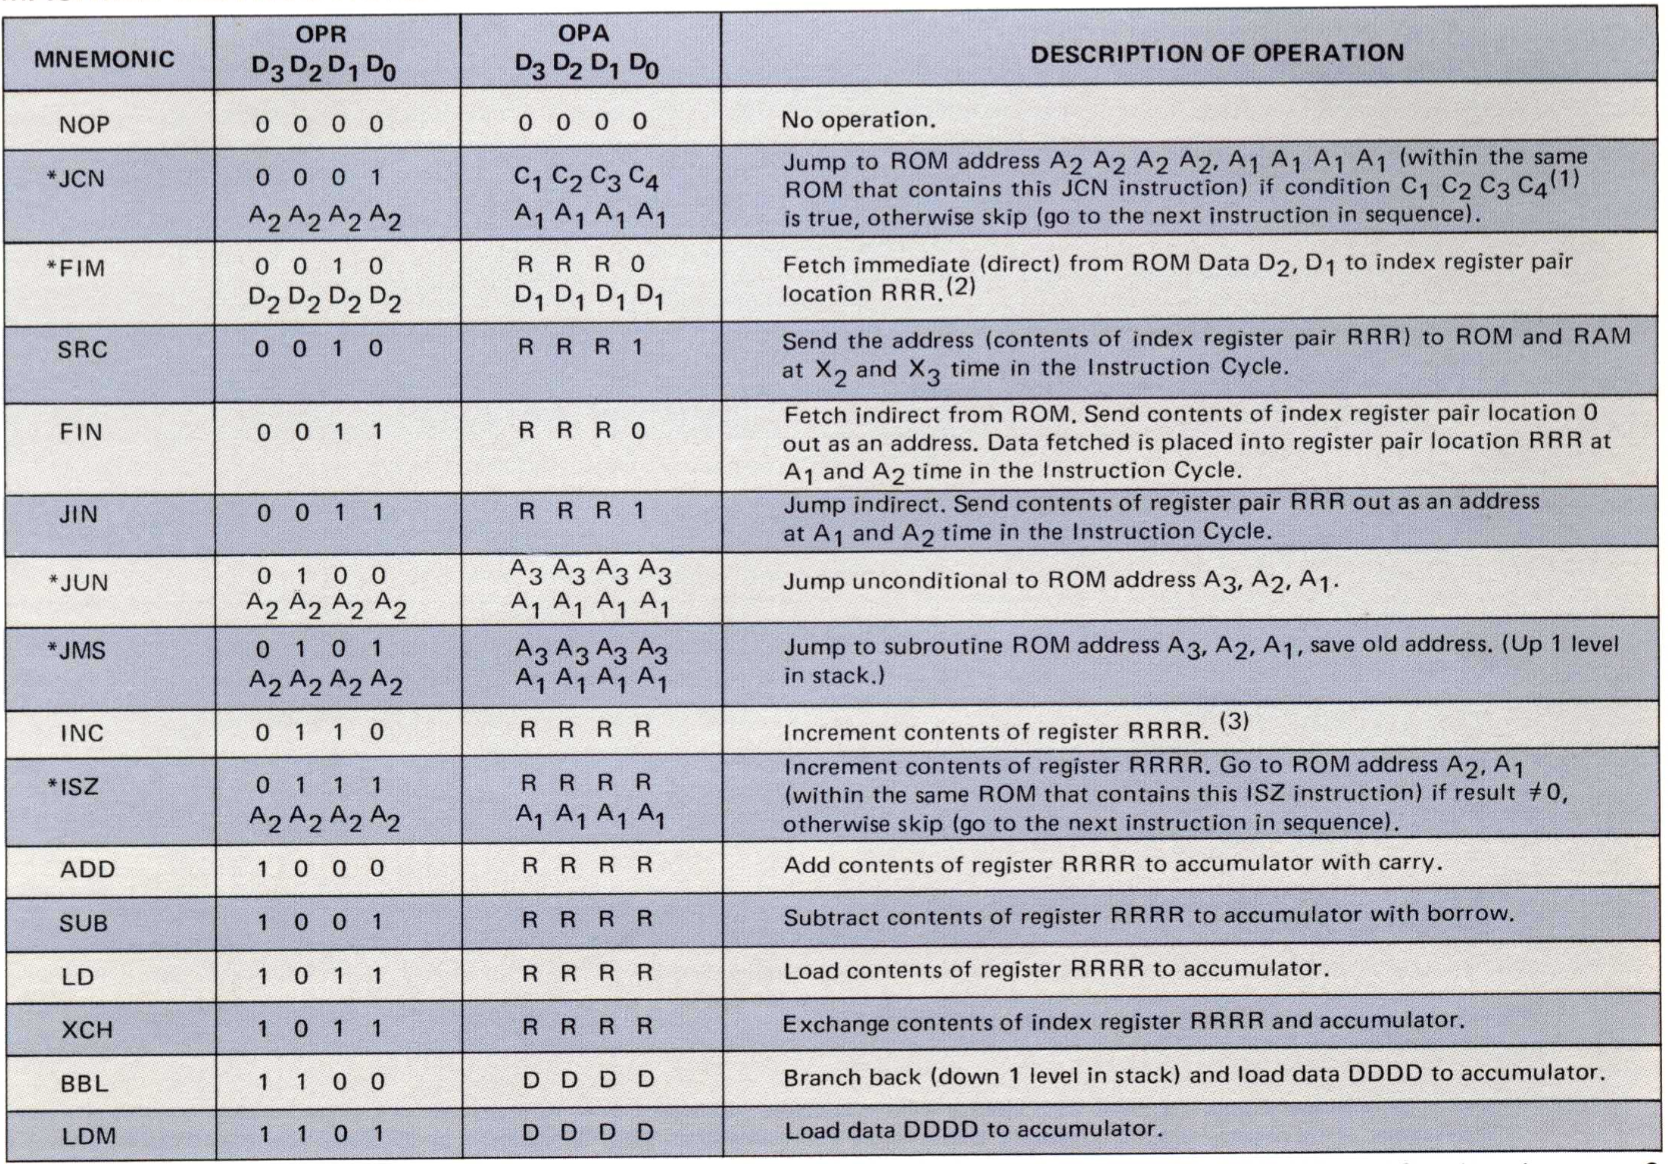
\includegraphics[width=0.8\linewidth]{images/instruction_machine.png}
	\end{figure}
\end{frame}

\begin{frame}
	\frametitle{Intel 4004 Spezifikation}
	\begin{itemize}
		\item Technik: PMOS Transistoren
		\item Strukturbreite: 10$\mu$m
		\item Transistorzahl: 2300
		\item Taktfrequenz: 740 KHz
		\item Dauer eines Befehlszyklus: 10.8 $\mu$s
		\item 92000 Befehle pro Sekunde
		\item Addition 2er 8 stelligen Zahlen: 850 $\mu$s
	\end{itemize}
\end{frame}

\subsection{Auswirkungen auf die Prozessorentwicklung}
\begin{frame}
	\frametitle{Auswirkungen auf die Prozessorentwicklung}
	\begin{itemize}
		\item Intel zögert Rechte von Busicom zurückzukaufen, da Prozessormarkt zu klein
		\item {\grqq}Revolution{\grqq} erst nachdem Intel weitere Developer Tools zur Verfügung stellt
		\item Weiterproduziert bis 1986
		\item Basis für den Intel 8080
		\item Intel hat heute einen Marktanteil von 80$\%$ bei PC-Mikroprozessoren
	\end{itemize}
\end{frame}

\begin{frame}
	\frametitle{Geschichte des MCS-4}
	\framesubtitle{1971 - MCS-4 Werbung}
	\begin{figure}[ht]
		\includegraphics[width=0.9\linewidth]{images/intel_ad.png}
	\end{figure}
\end{frame}

